\documentclass[10pt,letterpaper]{article}

\usepackage[margin=0.75in]{geometry}
\usepackage{tikz}
\usepackage{graphicx}
\usepackage{amsmath}
\graphicspath{{img/}}
\begin{document}

  \title{Stats 314, Data Analysis \#5}
  \author{Cody Malick\\
  \texttt{malickc@oregonstate.edu}}
  \date{\today}
  \maketitle

\section*{Part I}
\subsection*{a}
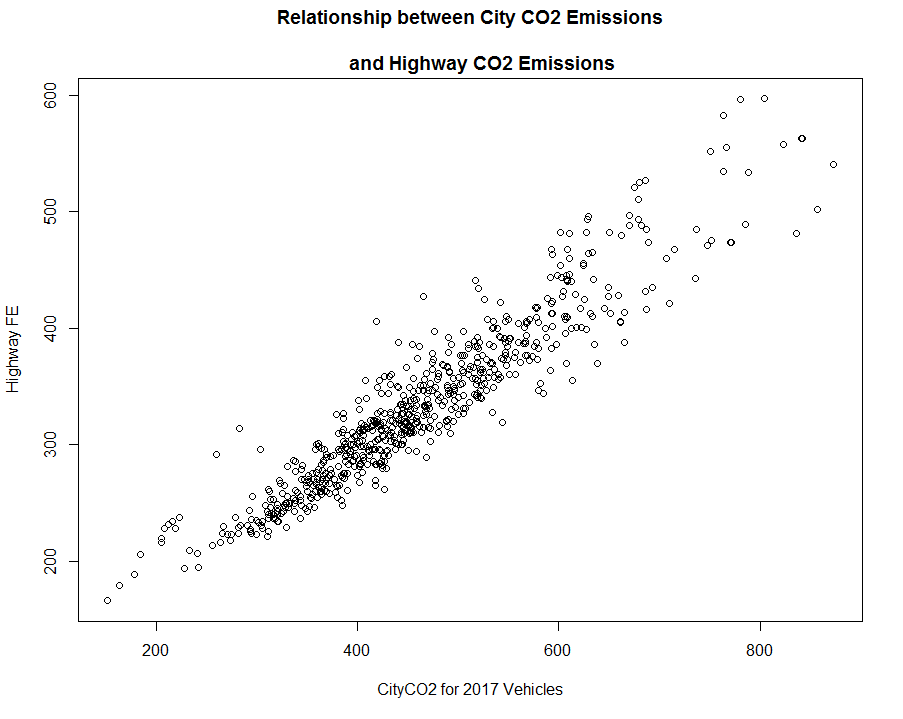
\includegraphics[scale=.6]{scatterplot}\\
There seems to be a moderately strong, positive, linear relationship between
City CO2
emmisions and Highway CO2 emmisions. There are a few positive outliers near the
center of the scatterplot, and a balanced number of positive and negative outliers
near the top right of the plot.


\subsection*{b}
The correlation coefficient:\\
$r=.9418$\\
The coeffcient measures the linear association strength between two quantative
variables. In this case, it is showing there is a fairly strong linear relationship
between city CO2 emissions and highway CO2 emissions.

\subsection*{c}
Residuals:\\
    Min      1Q  Median      3Q     Max \\
    -67.808 -14.695  -3.553  12.483  97.856\\ 

    Coefficients:\\
                 Estimate Std. Error t value Pr($>|t|$)\\    
		 (Intercept) 66.325785   3.411020   19.45   $<2e-16$ ***\\
		 CityCO2      0.577132   0.007082   81.50   $<2e-16$ ***\\
		 ---\\
		 Signif. codes:  0 *** 0.001 ** 0.01 * 0.05 . 0.1   1\\
\\
		 Residual standard error: 23.79 on 846 degrees of freedom\\
		 Multiple R-squared:  0.887,Adjusted R-squared:  0.8869 \\
		 F-statistic:  6642 on 1 and 846 DF,  p-value: $< 2.2e-16$\\
\\
Least squared regression line: $\hat{y} = b_0 + b_1 x$\\
$\hat{y} = 66.325+.5771x$

\subsection*{d}
\subsubsection*{i}
$H_0 \colon B_1 = 0$\\
$H_a \colon B_1 \neq 0$\\

\subsubsection*{ii}
$Test Statistic = \frac{.5771-0}{.007082}$\\
$81.488$\\

$p-value=.00000025$
\subsubsection*{iii}
The relationship between City CO2 emmisions and Highway CO2 looks to be convincingly
strong, with a correlation of .94. As City CO2 increases, highway CO2 also increases.
The relationship is modeled by the least squares regression equation:\\
$average emissions = 66.325 + .5771x$\\
Average city CO2 emissions is a significant predictor for Highway CO2 emissions
(t test stat = 81.5, df=846, and p-value .00000025).\\
The null hypothesis is rejected at a significant level of .01. The data supports
the assumptions that increasing city emissions may increase highway CO2 emissions.
The highway CO2 emissions are expected to increase .5771 for every 1 City CO2 emission
increase. 

\subsection*{e}
The slop shows how much the highway CO2 levels rise with the increase of city
CO2 levels. With a 99\% confidence interval from .5588 to .5954. That means
with 99\% confidence, we believe that the highway CO2 emissions increase
by .5771 for each 1 increase in City CO2 emissions. 

\subsection*{f}
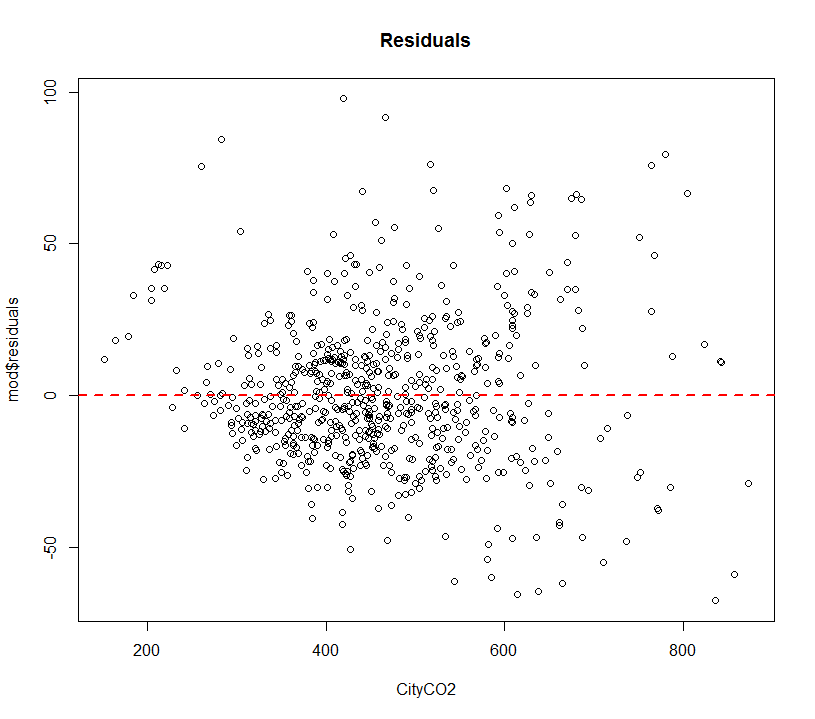
\includegraphics[scale=.6]{residuals}\\
The conditions for a residual graph are:\\
No distinct patters: Met\\
Roughly Scattered around Zero: Met\\


\subsection*{g}
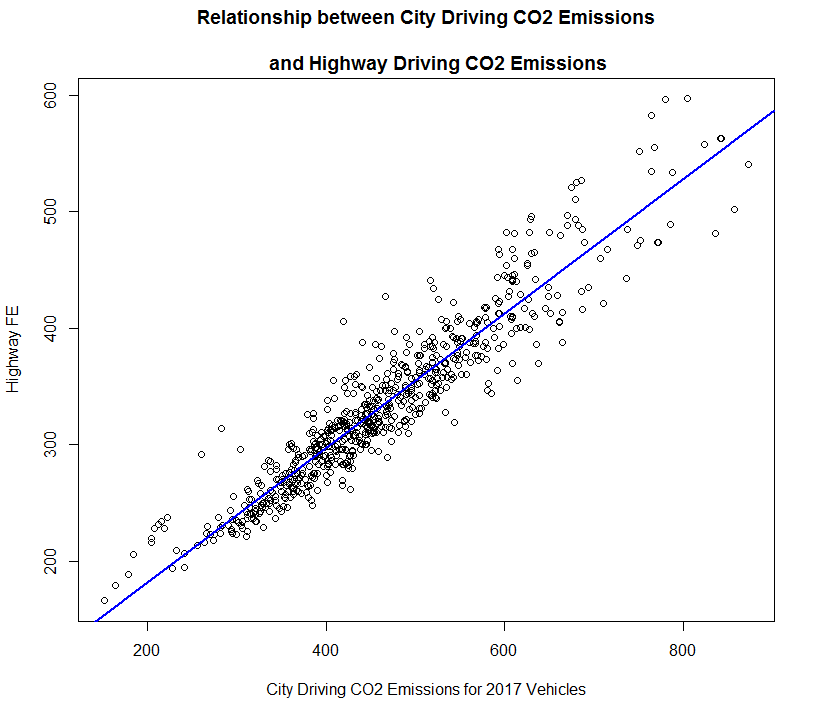
\includegraphics[scale=.6]{relationship}

\section*{Part II}
\subsection*{a}
Least squared regression line: $\hat{y} = 66.325+.5771x$\\
Plug in our value: $\hat{y} = 66.325 + .5771 * 550 = 383.73$

\subsection*{b}
Predicted: $383.73$\\
Observed: $389$\\
The difference between the observed and predicted is $5.27$

\subsection*{c}
The lower bound of our confidence interval is 381.1569\\
The upper bound of our confidence interval is 386.3398\\
The best fit for the interval is 383.7483\\

The upper and lower bounds are the 99\% confidence interval range, with an
estimated value of 383.7483.

\subsection*{d}
The lower bound of the prediction interval is 322.2737\\
The upper bound of the prediction interval is 445.223\\
The best fit for the prediction interval is 383.7483\

The upper and lower bounds are the 99\% prediction interval range, with an
estimated value of 383.7483.

\subsection*{e}
The difference between a prediction interval and confidence interval is the
standard error. The standard error in a prediction interval takes into account
the variability due to random sampling.

\section*{Part III}
\subsection*{a}
\begin{center}
	\begin{tabular}{| l | c | c | c | c | r |}
		\hline
		Source & Degrees of Freedom & Sum of Squares & Mean Squares & F & p-val \\ \hline
		Regression & 3 & 0.2013 & .0671 & 15.9052 & $<.0001$\\ \hline
		Residual & 17 & 0.0675 & .00421875  & & \\ \hline
		Total & 20 & 0.2688 & & & \\ \hline
	\end{tabular}
\end{center}
\subsection*{b}
$R^2=\frac{SSR}{SST}=\frac{.2013}{.2688}=.7488$\\
This value gives us the total proportion of our data that can be explained by the model.
In this case, that's roughly 75\%

\subsection*{c}
\subsubsection*{i}
$H_0:B_1=B_2=B_3$\\
$H_a:$ At least one $B$ is significant
\subsubsection*{ii}
$F=\frac{R^2/k}{(1-R^2)/(n-(k+1)}=\frac{MSR}{MSE}=\frac{.0671}{.00421875}=15.905$\\
Numerator degrees of freedom:3 \\
Denominator Degrees of Freedom:17 \\
p-value:$>.0001$ \\

\subsubsection*{iii}
There is at least one significant factor

\subsection*{d}
Least squares regression model $ = -.6799 - .00293x_1 - .00157x_2 + .06471x_3$

\subsection*{e}
$1.008747$ ppm 

\end{document}
